\subparagraph*{Problem explaination}
The problem is to learn the optimal price of the first item, especially comparing the adoption of a Thompson-sampling approach and an upper-confidence bound approach, in the following scenario:
\begin{itemize}
	\item Assignment of promos is fixed
	\item Price of second item is fixed
	\item Number of users per class is known
	\item Conversion rate associated with second item is known
	\item Prices are the same for all the classe
	\item Conversion rates do not change
\end{itemize}
\subparagraph*{Strategy}
The problem described is a combinatorial bandit problem,which is a decision making problem in which the decision maker selects one single arm in each round, and observes a realization of the corresponding unknown reward distribution. Each decision is based on past decisions and observed rewards. The objective is to maximize the expected cumulative reward over some time horizon by balancing exploitation and exploration. We can solve it, through an online algorithm, where only for the feasible solutions we will have precise estimations. We implement a script that works on a time horizon of ten days, repeating the experiment ten times. We simulate a random arrival of the customers, providing to them the prices given by the two learners (UCB and TS) for the first item and simulating the purchase of it. In case the customer buys the first item, we retrieve the reward of the second item as the product  between the conversion rate of that customer and the respective discounted price  We calculate the expected reward and we update the learners with the results. 
\subparagraph*{Upper-Confidence Bound (UCB1)}
Main idea:
\begin{itemize}
	\item Every arm is associated with an upper confidence bound 
	\item At every round, the arm with the highest upper confidence bound is chosen
	\item After having observed the realization of the reward of the arm, the upper confidence bound is updated
\end{itemize}
Notation:\\
\begin{itemize}
\item $t$ time
\item $A$ set of arms
\item $a$ arm
\item $a_{t}$ arm played at time $t$
\item $a^*$ optimal arm
\item $X_{a}$ random variable (bernoulli) associated to arm a
\item $\mu_{a}$ expected value of random variable $X_{a}$
\item $x_{a,t}$ realization of rv $X_{a}$ at time $t$
\item $x_{a}$ realizations of $X_{a}$
\item $\bar{x}_{a}$ empirical mean of $x_{a}$
\item $n_{a}(t)$ number of samples of arm $a$ at time $t$
\end{itemize}

Pseudocode\\

1. Play once each arm $a \in A$

2. At every time $t$ play arm $a$ such that:

$a_{t} \leftarrow \argmax_a{\left\{\left[\bar{x}_{a} + \sqrt{\frac{2 log(t)}{{n_{a}(t-1)}} }\right]\times a\right\}}$

\subparagraph*{Thompson Sampling (TS)}
Main idea:
\begin{itemize}
	\item For every arm, we have a prior on its expected value 
	\item In the case the arms’ rewards are Bernoulli distribution, the priors are Beta distributions
	\item Notice that, with the opportune parameters, a Beta distribution is a uniform distribution 
	\item For every arm, we draw a sample according to the corresponding Beta
	\item We choose the arm with the best sample 
	\item We update the Beta distribution of the chosen arm according the observed realization
\end{itemize}

Notation (in addition to classical UCB):\\
\begin{itemize}
	\item $\mathbb P(\mu_{a}=\theta_{a})$ prior of the expected value of $X_{a}$
	\item $\theta_{a}$ variable of $\mathbb P(\mu_{a}=\theta_{a})$
	\item $(\alpha_{a_{t}}, \beta_{a_{t}})$ parameters of the beta distribution $P(\mu_{a}=\theta_{a})$
\end{itemize}

Pseudocode\\

1. At every time $t$ for every arm $a$:

$\tilde{\theta_{a}} \leftarrow Sample(\mathbb P(\mu_{a}=\theta_{a}))$ \\

2. At every time $t$ play arm $a_{t}$ such that 

$a_{t} \leftarrow \argmax_a \left\{ \tilde{\theta_{a}} \times a \right\} $ \\

3.  Update beta distribution of arm $a_{t}$

$(\alpha_{a_{t}}, \beta_{a_{t}}) \leftarrow (\alpha_{a_{t}}, \beta_{a_{t}}) + (x_{a_{t},t}, 1 - x_{a_{t},t})$


\subparagraph*{Results}
\begin{center}
	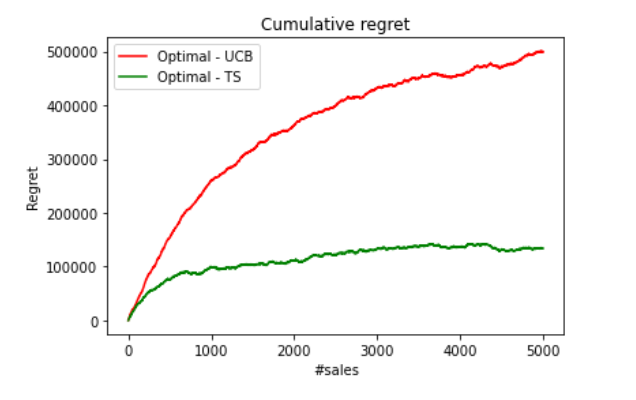
\includegraphics[scale=1.2]{Images/n3}
\end{center}
\subparagraph*{Considerations}
The result shows that a Thompson Sampling approach performs better than a UCB approach in our scenario, because the first have a lower regret than the second. Furthermore, we can also observe that the Thompson Sampling is faster to find the best price for the first item than UCB, because the TS regret curve becomes stable before UCB regret curve becomes stable.